\chapter{Results and Discussions}
The results and discussion for each solution considers the time taken for
operations to complete on each of the entities  as described in the University
example adopted for the experiments.

Each operation that triggers the referential integrity validation for an entity
namely the \texttt{insert}, \texttt{update}, \texttt{delete} operations are
measured in terms of time taken to complete the operation which includes
accessing and retrieving metadata  and the validation performed by the
\texttt{ValidationHandler}. The measured time is thus the response time the mean
average for the operations.

Section~\ref{sr:baseline} presents the results for the baseline testbed where no
referential validation checks are implemented and the operations performed on
the entities are just as it would be performed in Cassandra without any
referential integrity validation.


\section{Baseline}\label{sr:baseline}
A baseline measurement to assess the performance of the implemented solutions is
presented in Figure~\ref{fr:Solution0-barplot}.
The factors measured were the time involved to complete each operation for every
entity, where the operations considered were the ones that invoked referential
integrity validation, namely, \texttt{insert}, \texttt{update} and
\texttt{delete}. These were measured for the entities in the University example,
namely \texttt{Student}, \texttt{Course} and \texttt{Enrolment}.
% The results are plotted as a histogram in Figure~\ref{}
	
\begin{figure}[h] \centering
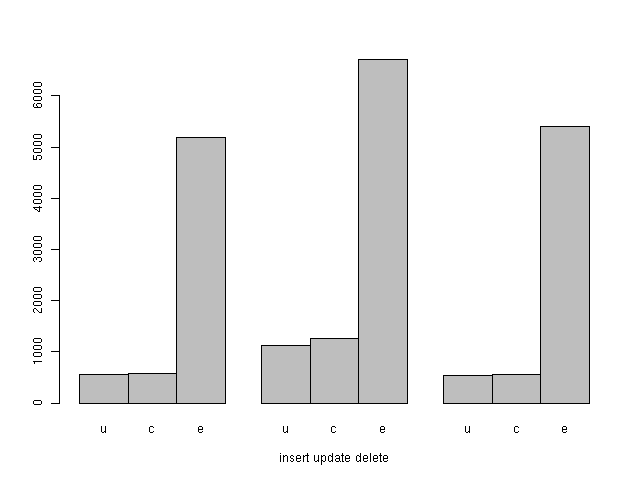
\includegraphics[width=.8\textwidth]{./figure/result/Solution0-barplot.png}
		\caption{Baseline}\label{fr:Solution0-barplot}
	\end{figure}
	
% Present results.
	The potential reasons for the variance of time for the completion of each
	operations on the different entities are summarised next.
	\begin{description}
	\item[Insert] The time for inserting entities into the \texttt{Student} and
	\texttt{Course} column families are similar since the number of entities are
	exactly the same.
	\texttt{1000} instances of \texttt{Student} and \texttt{Course} are inserted
	into the respective column families for the baseline test. The time taken to
	insert the \texttt{Enrolment} entities into the \texttt{Enrolment} column family
	is higher by approximately \texttt{4} seconds. This is because
	\texttt{enrolment} has more entities, to be specific, it has \texttt{10,000}
	instances. Hence, the \texttt{insert} operation takes more time to insert
	entities into \texttt{Enrolment} column family, especially considering its
	replication across \texttt{10} nodes, which would add to the time in
	completing the operation.
	
	\item[Update] The time for updating the primary keys in \texttt{Student} and
	\texttt{Course} are comparable to each other. Although the number of entities
	updated are the same, the small difference is owing to external variables
	(e.g. network latency, network traffic). Similar to the \texttt{insert}
	operation, updating the \texttt{Enrolment} entities takes significantly more
	time, which is again due to the higher number of entities held within this
	column family. The time for \texttt{update} operation on \texttt{Enrolment} is
	higher when compared to the time taken for \texttt{insert} operation on the
	same. This is mainly due to the additional computational resources consumed to
	ensure the existence of an entity before updating it to new values.
	
	\item[Delete] The time involved for completion of the \texttt{delete} operation
	on all the entities from \texttt{Student} and \texttt{Course} column families are
	similar to each other, owing to the same number of entities and similar
	replication strategies. This is similar to the \texttt{insert} operation in
	terms of time taken for completion and the processes involved. This means that
	unlike \texttt{update} both \texttt{delete} and \texttt{insert} do not
	involve additional operations and simply adds or removes entities from the
	column families.
	The time involved for the \texttt{delete} operation to delete all the entities
	in \texttt{Enrolment} is higher just as in other operations. This is again due
	to the larger number of entities present in \texttt{Enrolment}.
	\end{description}

	
	
% 	Explain Insert. Why student and course similar. Why enrolment much higher.
% 	

	In general, all the operations take more time to complete on the
	\texttt{Enrolment} column family due to the larger number of entities stored
	when compared to \texttt{Student} and \texttt{Course} column families. the
	\texttt{update} operation consumes more time due to the additional search
	involved to locate the previous state of the entity prior to updating it to new
	values. Notice that the time involved to complete \texttt{insert} and
	\texttt{delete} entities form all the three column families are similar.
	
	In the following sections the performance of each solution is discussed in
	terms of referential integrity validation in each of the \texttt{insert},
	\texttt{update} and \texttt{delete} operation.
	
\section{Insert}\label{sr:insert}
An \texttt{insert} operation triggers a referential integrity validation
whenever a child entity containing foreign keys is inserted. This means that
each time a child entity is inserted the \texttt{ValidatoinHandler} in all the
solutions validates that the foreign keys exist as primary keys in the parent
entities. This dependency information is retrieved from the metadata saved in
each solutions. During the experiments, the time taken to insert all the
entities are recorded and this includes the time involved for validating
referential integrity for the entity. Across all the solutions in the
experiments, the \texttt{insert} operation triggers such a validation when the
\texttt{Enrolment} entities are inserted since it is a child entity containing
foreign keys of \texttt{student} and \texttt{course} entities. As mentioned in
Section~\ref{s:exp:setup} the number of entities inserted into the
\texttt{Enrolment} column family is the same for all solutions. Despite the same
number of entities and similar validation performed, the time consumed for this
operation in all the solutions are different and is further analysed.
		
It can be seen from the histograms of the solutions that all the solutions take
similar amount of time to insert entities into \texttt{Student} and
\texttt{Course} column families. This is because there are no referential
integrity validation involved in inserting these entities since these entities
do not contain any foreign keys. On the other hand the time consumed to insert
\texttt{Enrolment} entities varies across the solutions since there is
referential integrity validation where metadata constraints are read and
validated.
The results show that Solutions~1 and 4 take approximately 15 seconds to insert
entities into \texttt{Enrolment} while Solution~2 takes lesser than 35 seconds. Solution~3
takes slightly more than 35 seconds and takes the most time to insert the
records into the \texttt{Enrolment} column family when compared to all the other
solutions and the baseline. This is mainly due to the way metadata is accessed
and read from an external location or a different column family in this
solution. The validation involves accessing the  columns of the
\texttt{Metadata} column family in this solution to get each value of the
constraint.
		
Performing the \texttt{insert} operation for the 10000 entities in
\texttt{Enrolment} is thus more time consuming for all the solutions when
compared to inserting entities into other column families and this is similar to
the baseline experiment where inserting \texttt{Enrolment} entities was more
time consuming.
However in the solutions, the time taken to insert entities into
\texttt{Enrolment} is higher when compared to the same in the baseline tests and
this is  due to the referential validation that is triggered while inserting
child entities in the solutions. However, it is evident that despite the
different way of storing metadata both Solutions~1 and 4 perform better than the
rest of the solutions to perform such a validation on \texttt{insert}.

\newpage
\section{Update}\label{sr:update}
In all the solutions, the \texttt{update} operation triggers a referential
integrity validation whenever an entity is updated. Moreover, data manipulation
rules are also applied which specifies whether the \texttt{update} is a
\texttt{Cascade} or \texttt{NoDelete}. The \texttt{ValidationHandler} of all the
solutions perform these validations and accesses metadata and its various parts
to determine whether the referential integrity is violated or not. This is
unlike the baseline where there are no referential integrity validations and any
value is allowed to be changed without checking its correctness or validity. In
all the solutions the time taken to update the primary keys in \texttt{Student}
and \texttt{Course} and time taken to update the foreign key \texttt{CourseId}
in \texttt{Enrolment} is measured and this is different for each solution.The
performance of the solutions in the different cases involved in \texttt{update}
is discussed next.

	\begin{itemize}
	  \item Updating \texttt{Student} entities involve cascading the changes within the
	child entity \texttt{Enrolment}.
	%  while updating \texttt{Course} throws an
	% exception since \texttt{course} entities have a \texttt{NoDelete} manipulation
	% rule in its metadata, thus preventing the \texttt{update}. 
	Both Solutions~1 and 4 take slightly more than
	25 seconds to perform a cascaded \texttt{update} for \texttt{Student} entities.
	Solution~2 takes slightly more than 20 seconds and takes lesser time than other
	solutions, while Solution~3 takes the most time of more than 60 seconds. All the
	solutions takes more time to insert \texttt{Student} entities when compared to
	the baseline due to the referential integrity validation and the cascaded
	operations, which additionally accesses \texttt{Enrolment} to complete the
	\texttt{update} operation.
	
	  \item Updating \texttt{Course} entities involves identifying the metadata
	constraints and raising an exception due to the \texttt{NoDelete} rule applicable for every
	\texttt{Course} entity, which prevents the \texttt{update} operation. From the
	results it can inferred that both Solutions~1 and 4 take the least time amongst
	all solutions, where Solution~1 takes less than 5 seconds and Solution~4
	close to it. Solution~2 is not far behind form these solutions and
	takes slightly more than 5 seconds, but Solution~3 takes twice the amount of
	time than the rest of the solutions to update the \texttt{Course} entities.
	When compared to the baseline, updating \texttt{Course} takes more time in all
	solutions since  validations are triggered and  exceptions raised unlike the
	baseline. The only difference between this operation in the solutions and
	the baseline is the time involved in the validation and handling the
	exceptions.
	
	\item When \texttt{Enrolment} is updated the values are changed only within the
	\texttt{Enrolment} column family but \texttt{Student} and \texttt{course}
	families are accessed to verify the validity of the foreign keys.The results
	show that Solutions~1 and 4 almost take the same time of slightly more than 15
	seconds, while Solution~2 takes more than 35 seconds. Solution~3 takes the most
	time which is slightly less than 40 seconds. 
	\end{itemize}
Generally, in all the solutions updating the \texttt{Course} entities take the
least time when compared to updating \texttt{Student} or \texttt{Course}
entities.
This is because \texttt{update} for \texttt{Course} entities trigger validation
but does not involve updating the entities nor are any cascade operations performed.
The time involved in updating \texttt{Enrolment} is lesser than updating the
\texttt{Student} entities since it does not involve cascading operations but
updates only values within itself and limits the validation to only accessing
the parent entities to ensure the existence of the foreign keys. This takes more
time than \texttt{update} on \texttt{Course} since updating \texttt{Enrolment}
involves changing the values after the validation and accessing the parent
entity classes for validation unlike \texttt{update} on \texttt{Course} where
validation takes place but no other column families are accessed nor are values
changed. It is interesting to note that in 	Solution~2 the time for updating the
\texttt{Enrolment} entities is more than updating \texttt{Student} entities
unlike all the solutions. This is mainly because an \texttt{update} involves an
\texttt{insert} and \texttt{delete} operation. It can be seen that this
\texttt{update} on \texttt{Enrolment} is similar to the time taken to
\texttt{insert} the \texttt{Enrolment} entities in this solution. The difference
in the way metadata is stored and retrieved is also another cause for this
anomaly and is further explained in Section~\ref{}.


\section{Delete}\label{sr:delete}
In all the solutions, the \texttt{delete} operation triggers a referential
integrity validation whenever a parent entity is deleted. Just as in an
\texttt{update}, data manipulation rules are  applied specifying whether the
\texttt{delete} is a \texttt{Cascade} or \texttt{NoDelete}. In all the solutions
the time taken to delete the entities  are recorded and experiments are designed
to test every case of the \texttt{delete} operation. This means that both
cascaded deletes of \texttt{Student} entities and deletions of
\texttt{Course} entities with no dependencies are tested. The performance of the
solutions in these different cases involved is discussed next.

\begin{itemize}
  \item Deleting \texttt{Student} entities involved  deleting  the \texttt{Enrolment} 
  entities that had foreign keys of \texttt{Student}. This cascaded delete was
  determined from the \texttt{DeleteRule} of the \ac{PK} constraint of \texttt{Student} entities.
%   this operation involved deleting \texttt{enrolment} entities that had the
%   \texttt{StudentId} of the \texttt{Student} entity marked for deltion as a
%   foreign key. 
  In this case, the time measured involved the cascaded delete of
  entities from \texttt{Enrolment} and then the deletion of the \texttt{Student}
  entity from the \texttt{Student} column family. From the results it can be
  summarised that Solutions~2 and 4 performed similarly and took slightly more
  than 15 seconds. Solution~1 took the least amount of time with less than 10
  seconds and Solution~3 took more than 20 seconds to complete the cascaded
  deletion.When compared to the baseline, all the solutions take considerably
  longer to perform the \texttt{delete} on \texttt{Student} entities. This is
  because of the referential integrity validation and the cascaded operations.
  Like \texttt{update} this operation also accesses another column family to
  complete the operation.
  
  \item Deleting the \texttt{Course} entities also invoked referential
  integrity validation and despite its \texttt{NoDelete} rule, \texttt{Course}
  entities that had no current dependencies in \texttt{Enrolment} were deleted
  and the time measured. The results show that Solutions~1 and 4 take
  approximately 2 seconds while Solutions~2 and 3 take slightly less than 5
  seconds.When compared to the baseline this operation generally takes slightly
  longer. This is because prior to the deletion of the entities all solutions
  perform the validation and checks the metadata. The operation then deletes the
  entities when no child dependencies exist.
  
  \item Deleting \texttt{Enrolment} invokes no validation although the metadata
  is checked for the entity. Solutions~1 and 4 take slightly more than 5
  seconds to complete this operation while Solution~2 takes more than 10
  seconds. Solution~3 takes more than 20 seconds to complete the operation and
  is the longest when compared to the other solutions. When compared to the
  baseline, the solutions take longer to complete despite having no referential
  integrity constraints. This is because when the \texttt{delete} operation is
  invoked on \texttt{Enrolment} it is treated as any other entity and its
  metadata is accessed and \texttt{ValidationHandler} determines if any
  \ac{FK} constraints exist for it.
  
\end{itemize}

In general, deleting \texttt{Student} entities take the longest time in all the
solutions unlike the baseline. The time is higher due to the validation and the
cascaded operation which accesses another column family in the cluster. The
\texttt{delete} on \texttt{Enrolment} is lower than \texttt{delete} on
\texttt{Students} because \texttt{Enrolment} has no dependencies and the
validation involves checking whether it has any child dependent on it. Apart
form this metadata checking, the entities are deleted just as in the baseline.
The operation is shortest when \texttt{Course} entities are deleted and is
because similar to deleting \texttt{Enrolment} validation is performed and the
delete takes place. It takes lesser time than deleting \texttt{students} because
data in other column families are not accessed or changed. Although similar to
\texttt{delete} on \texttt{Enrolment}, \texttt{Course} takes lesser time due to
its lesser number of entities when compared to \texttt{Enrolment} entities which
is 10 times more.



\newcommand{\Width}{.5\textwidth}
% 	Explain update. Student and course are similar, small difference to external
% 	variables (e.g. network latency). Same, enrolment is higher. Blame update
% 	higher times than insert due to additional computational resources spent
% 	ensuring the previous existence of the record before changing new values.
% 	
% 	Delete. Similar to insert. It does not require changing values, but just
% 	removing. However, notice that in average the differences between insert and
% 	delete are rather small, and both with respect to update are a bit bigger.

\begin{figure}
	\centering
	\subfigure[Solution1]{
	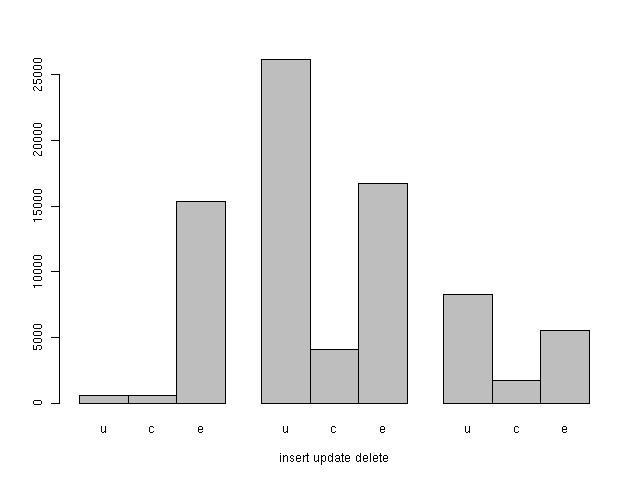
\includegraphics[width=\Width]{./figure/result/Solution1-barplot.png}
	}\subfigure[Solution2]{
	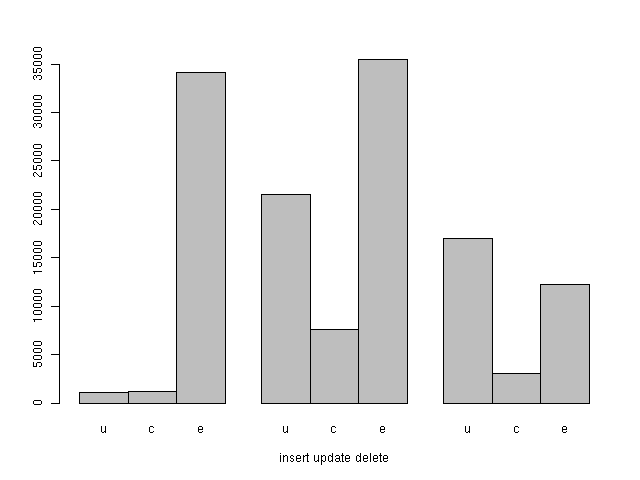
\includegraphics[width=\Width]{./figure/result/Solution2-barplot.png}
	}\\
	\subfigure[Solution3]{
	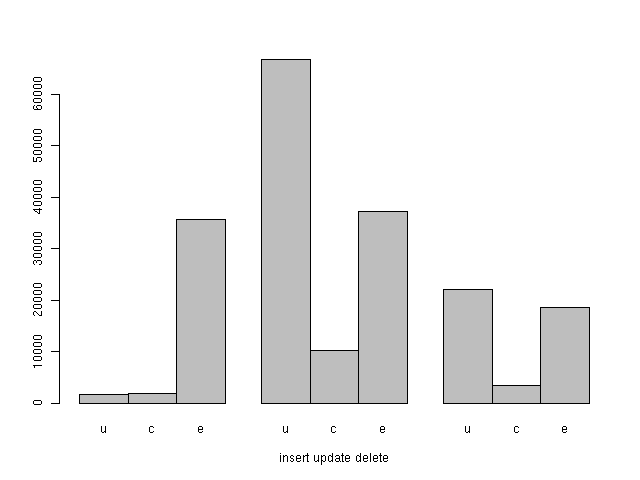
\includegraphics[width=\Width]{./figure/result/Solution3-barplot.png}
	}\subfigure[Solution4]{
	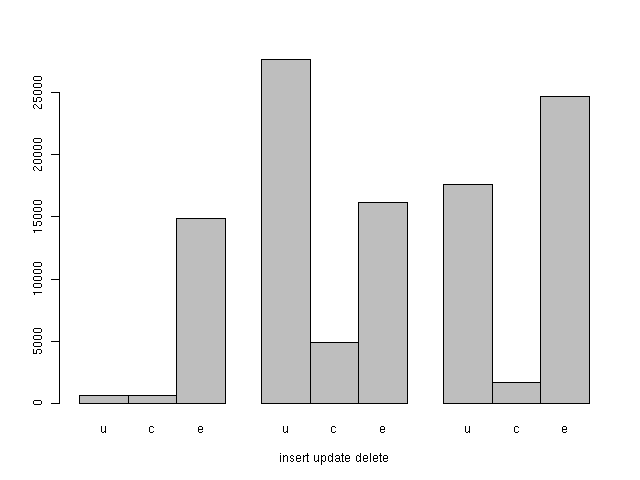
\includegraphics[width=\Width]{./figure/result/Solution4-barplot.png}
	}\\
	\subfigure[Baseline]{
	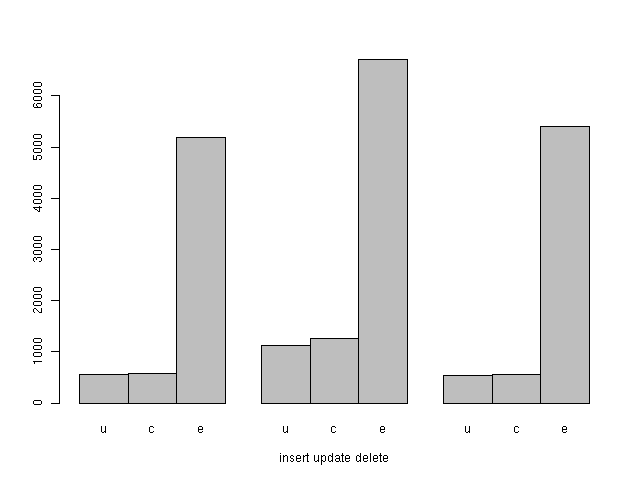
\includegraphics[width=\Width]{./figure/result/Solution0-barplot.png}
	}
\end{figure}


\renewcommand{\Width}{.6\textwidth}
\begin{figure}
	\centering
	\subfigure[User]{
	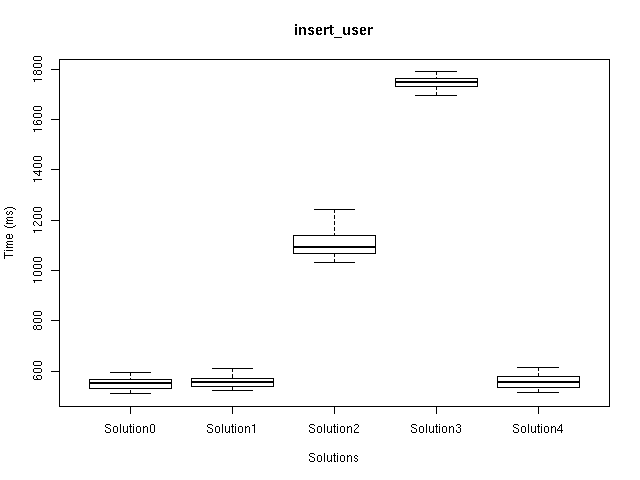
\includegraphics[width=\Width]{./figure/result/bp-insert_user.png}
	}
	\subfigure[Course]{
	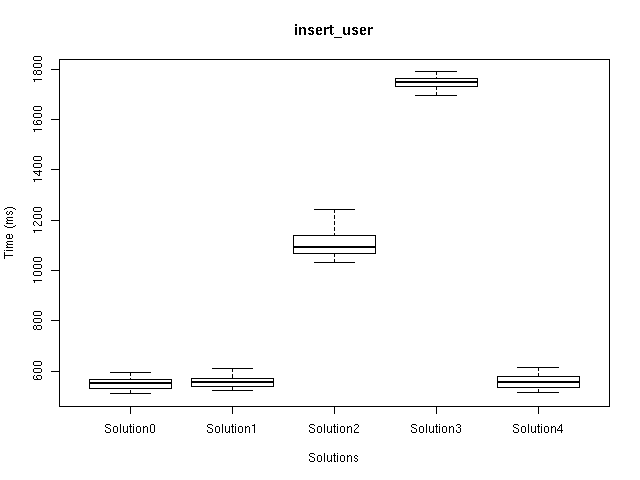
\includegraphics[width=\Width]{./figure/result/bp-insert_user.png}
	}
	\subfigure[Enrolment]{
	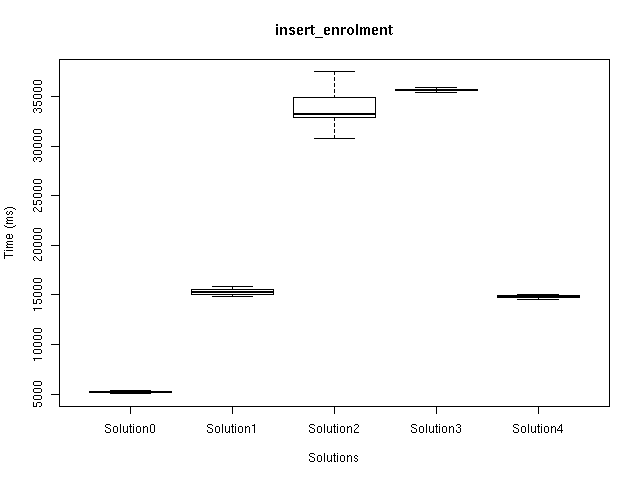
\includegraphics[width=\Width]{./figure/result/bp-insert_enrolment.png}
	}
	\caption{Insert}
\end{figure}


\begin{figure}
	\centering
	\subfigure[User]{
	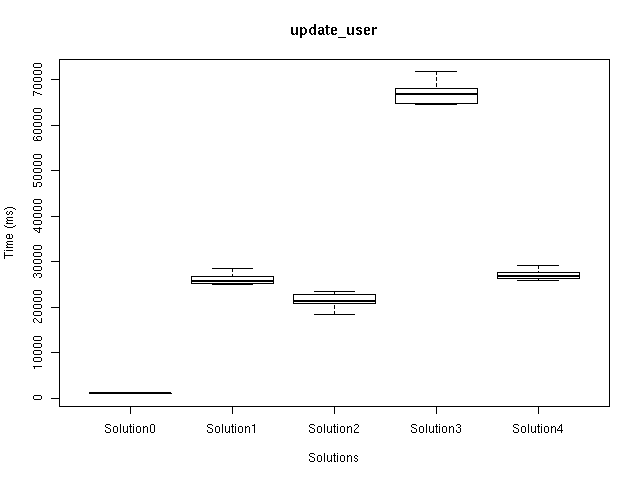
\includegraphics[width=\Width]{./figure/result/bp-update_user.png}
	}
	\subfigure[Course]{
	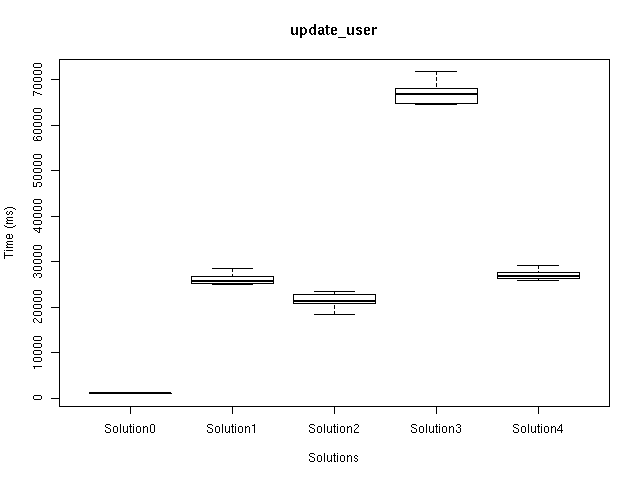
\includegraphics[width=\Width]{./figure/result/bp-update_user.png}
	}
	\subfigure[Enrolment]{
	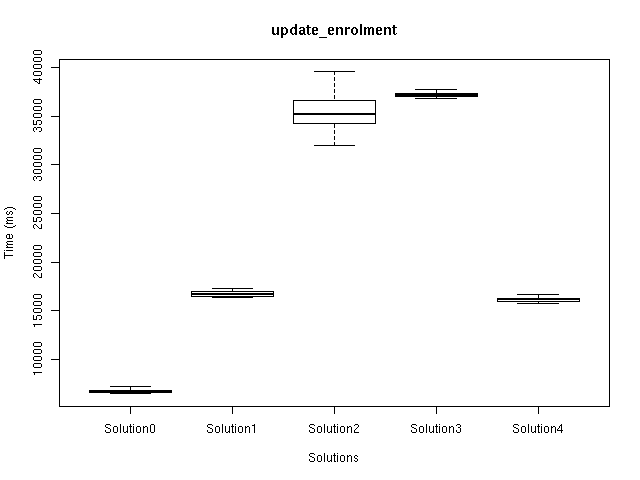
\includegraphics[width=\Width]{./figure/result/bp-update_enrolment.png}
	}
	\caption{Update}
\end{figure}


\begin{figure}
	\centering
	\subfigure[User]{
	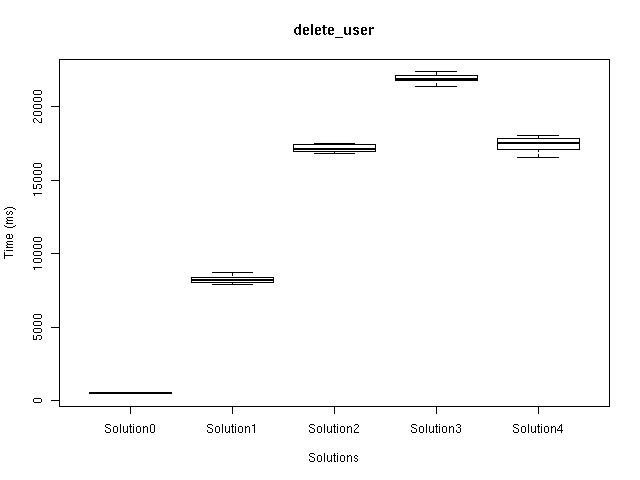
\includegraphics[width=\Width]{./figure/result/bp-delete_user.png}
	}
	\subfigure[Course]{
	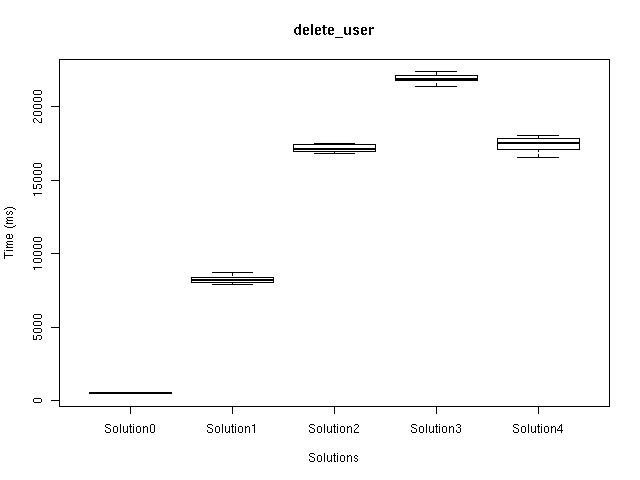
\includegraphics[width=\Width]{./figure/result/bp-delete_user.png}
	} 
	\subfigure[Enrolment]{
	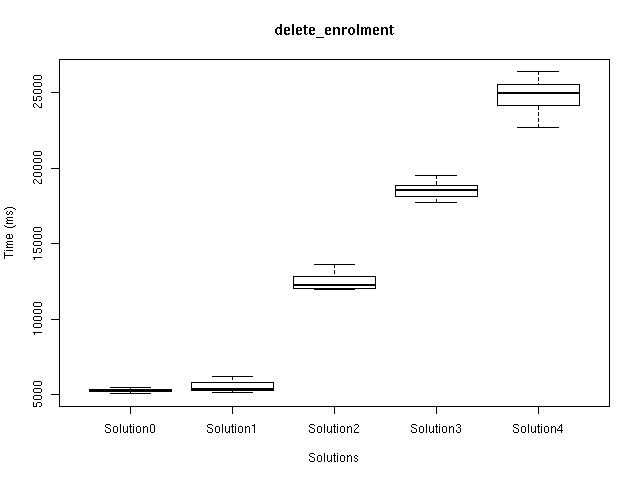
\includegraphics[width=\Width]{./figure/result/bp-delete_enrolment.png}
	}
	\caption{Delete}
\end{figure}

% \newcommand{\B}[1]{\colorbox{light-gray}{#1}}
% \begin{tabular}{ccccccc}
% \toprule
% &&Solution0 & Solution1 & Solution2 & Solution3 & Solution4\\
% \midrule
% \multirow{3}{*}{insert} & u & \rc 0.624 (0.138) & 0.614 (0.029) & 1.140 (0.057)
% & 3.444 (0.070) & 0.586 (0.039)\\
%  & c & 0.630 (0.069) & 0.621 (0.027) & 1.181 (0.087) & 3.447 (0.096) & 0.584 (0.030)\\
%  & e &  5.708 (0.310) & 16.883 (0.278) & 34.220 (1.399) & 55.359 (0.351) &
%  15.340 (0.276)\\
% \midrule
% \multirow{3}{*}{update} & u & 1.254 (0.051) & 32.312 (1.207) & 25.046
% (0.986) & 113.579 (1.495) & 48.000 (1.537)\\
%  & c &  1.376 (0.099) & 7.559 (0.297) & 10.885 (0.384) & 19.279 (0.252) &
%  7.580 (0.288)\\
%  & e & 7.237 (0.425) & 18.228 (0.276) & 35.673 (1.402) & 56.762 (0.420) & 16.694 (0.386)\\
% \midrule
% \multirow{3}{*}{delete} & u & 0.592 (0.022) & 10.798 (0.409) & 18.952
% (0.600) & 42.544 (0.619) & 35.919 (0.576)\\
%  & c & 0.627 (0.023) & 3.602 (0.092) & 4.828 (0.118) & 6.745 (0.120) & 3.324 (0.079)\\
%  & e & 5.847 (0.294) & 5.904 (0.359) & 12.282 (0.650) & 35.070 (0.472) & 57.647 (0.799)\\
% \bottomrule
% \end{tabular}

\section{Analysis of results}
